 \documentclass{article}
% \usepackage{geometry}
\usepackage[a4paper,top=3cm,bottom=2cm,left=3cm,right=3cm,marginparwidth=1.75cm]{geometry}
\usepackage{graphicx}
\usepackage[english]{babel}
\usepackage[utf8]{inputenc}
\usepackage{setspace}
\usepackage[T1]{fontenc}
\usepackage{amsmath}
\usepackage{csquotes}% Recommended
\usepackage{float}
\usepackage[caption = false]{subfig}
\usepackage[style=authoryear,backend=biber]{biblatex}
\doublespacing
\usepackage{lineno}
\linenumbers
\usepackage{longtable} %%%
\addbibresource{references}% Syntax for version >= 1.2
%

% title
\title{Functional Responses and Temperature}%
\author{Ruth Keane}
\begin{document}
\begin{titlepage}

\newcommand{\HRule}{\rule{\linewidth}{0.5mm}} 

\includegraphics[width=8cm]{logo.eps}\\[1cm] 
\center 

\textsc{\LARGE CMEE Miniproject}\\[1.5cm] 
\textsc{\Large Imperial College London}\\[0.5cm]
\textsc{\large Life Sciences}\\[0.5cm] 

\makeatletter
\HRule \\[0.4cm]
{ \huge \bfseries \@title}\\[0.4cm] % Title of your document
\HRule \\[1.5cm]
\makeatother
\Large \emph{Author:}\\
Ruth Keane \\[3cm] % Your name
\input{../Results/Tables/wordcount}\\

{\large \today}\\[2cm] % Date, change the \today to a set date if you want to be precise

\vfill % Fill the rest of the page with whitespace

\end{titlepage}

\begin{abstract}
this is the abstract.

\end{abstract}
%
%
%
\section{Introduction}
The functional response describes how predators respond to changes in prey density \parencite{hollingsawfly1959}\parencite{Solomon1949}. As prey numbers increase, the consumption rate of predators initially increases then levels out, however the specific shape of the period of increase can vary \parencite{hollingsawfly1959}. Holling modelled the functional response and suggested three different forms which worked for different types of organisms \parencite{hollingsawfly1959}. These are Type I, where the rate of increase in prey consumption with prey density is constant before the plateau, type II where the rate of increase in prey consumption with prey density is decreasing and type III, where the  rate of increase in prey consumption with prey density increases then decreases \parencite{hollingsawfly1959}. The type I model can be described by equation \ref{type1}, the type II model can be described by equation \ref{type3} where $x_R$ is the resource density, $c$ is the number of prey consumed per predator per unit time,$a$ is the discovery or search rate of the consumer and $h$ is the handling time \parencite{Dawes2013}\parencite{Holling1959}. The type III model can be described by a generalised version of equation \ref{type2}, equation \ref{type3} where $q$ changes the shape of the curve\parencite{Dawes2013}. %explain how - dawes? or unnecessary%
When $q=0$, the model is type II and when $q>0$,the model is type III \parencite{Dawes2013}. These equations are often written with $Y$, the number of prey consumed per predator, instead of $c$ and $T$, the time, on the right side of the equation, however these equations are equivalent as $c=\frac{Y}{T}$.%is this line helping?
\begin{equation}\label{type1}
    c=ax_R
\end{equation}
\begin{equation}\label{type2}
c=\frac{ax_R}{1+hax_R}
\end{equation}
\begin{equation}\label{type3}
c=\frac{ax_R^{q+1}}{1+hax_R^{q+1}}
\end{equation}
%Models in general %
Models can be phenomenological or mechanistic. %advantages and disadvantages
The Holling models described above are mechanistic however the type III model is more phenomenological due to the non-biological parameter $q$.
%%what effects the functional response 

%% What is my question
%
%
\section{Methods}
\subsection{Computing Tools}
%what packages were used and why
\subsection{Initial Data Sorting}
The data used was from the Biotraits database \parencite{Dell2013}, which contains information collated from different studies about how biological traits respond to environmental drivers. The parameters of interest here were the number of prey the predator consumed per unit time and the resource density. Data sorting was carried out in python version 2.7. New columns were added and experiments with less than six experiments were removed. This new dataset was exported to a csv for model fitting. The
\subsection{Model Fitting}
The data were fitted to five different models, a quadratic model, a cubic model and the three Holling models \parencite{Holling1959} using R 3.6.2 \parencite{RCoreTeam2017}. The Holling models were the type I model (equation \ref{type1}, a linear model), type II model (equation \ref{type2}) and generalised type III model (equation \ref{type3}).
Models were fitted sequentially for each experiment and plotted. This allowed the fit to be visually inspected as the model fitting process was improved.
\subsubsection{Linear models}
 The Holling type I, quadratic and cubic models models were fitted using lm (base R). For the quadratic and cubic models, poly was used to compute orthogonal polynomials to avoid correlation of variables.
\subsubsection{Non-linear Models}
The Holling type II and type III models were fitted using NLSlm (from the package minpack.lm \parencite{Elzhov2016}). The coefficients $a$, $h$, and $q$ were given a lower bound of zero and the maximum number of iterations was set to $1000$. For both type II and type III models, starting values were calculated using starting value functions where $a$, $h$ and $q$ were estimated, followed by sampling positive values around these initial values and repeatedly running the models and storing the coefficients and AIC values of these models. The coefficients of the model with the lowest AIC were used as the initial values for the main model fitting step. The initial value for $h$ was the maximum value of $c$. The initial value for $a$ was the initial steep part of the curve which was calculated by repeatedly fitting linear models the dataset then deleting the maximum value of $x_R$ and storing the largest gradient of these models.For the type III model, this initial value of $q$ was set at %pick and also justify
Once the starting values had been determined, the models were rerun with these initial values and plotted (with the other models). %try?
\subsection{Data Analysis}
%how many 
The models were compared using AIC and the most appropriate model was determined for each dataset. AIC was used because other techniques to compare models are not appropriate for non linear models.  %why AIC not bic
The confidence intervals for values of $q$ were calculated and (using two times the standard error). When the confidence interval for $q$ overlapped zero, the best AIC was recalculated for the remaining four models (because when the confidence interval for $q$ is zero, the type III model is the same as the type III model.  %%remove this?

%talk about stats stuff- tests 
\section{Results}
%figs will need to be saved into code directory probs
\subsection{Number of Fits}
Many of the Hollings model fit well to the data \ref{fig:2}. % don't love format for this , where should this go!
\begin{figure}[h] %h forces it to be at this location
    \centering
    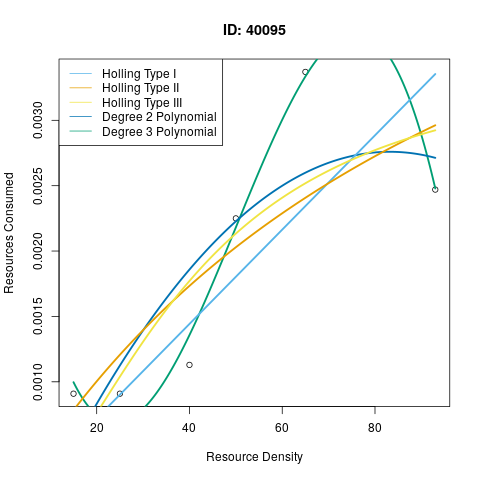
\includegraphics[width=5in]{../Results/Plots/40095}
    \caption{This is a graph for 40095}
    \label{fig:2}
\end{figure}
%best model, significance
\subsection{Best Model}
The Holling's type II model was most frequently the best model (29.5\%) and the polynomial of degree 2 was most frequently the second best model (31.5\%) (Figure \ref{fig:bestmodel}).
The mechanistic models were marginally more often the best model (53.1\%)than the mechanistic models (Figure \ref{fig:modelbesttype} )
\begin{figure}[h]
\centering
\subfloat[Number of times that each model was the best model]{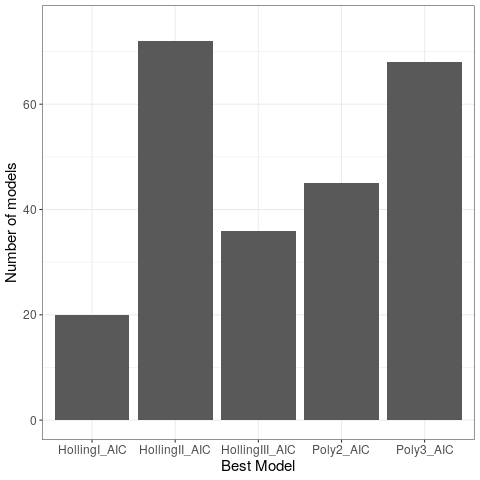
\includegraphics[width = 3in]{../Results/Plots/modelbest}}
\subfloat[Number of times that each model was the second best model]{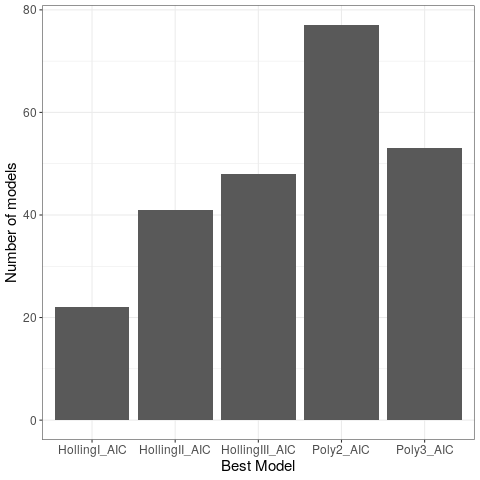
\includegraphics[width = 3in]{../Results/Plots/modelsecondbest}}
\caption{Best and second best model from the lowest and second lowest AIC values. Models are Holling type I, Holling type II, Holling type II, polynomial of degree 2, polynomial of degree 3. n=241}
\label{fig:bestmodel}
\end{figure}
\begin{figure}[h] %h forces it to be at this location
    \centering
    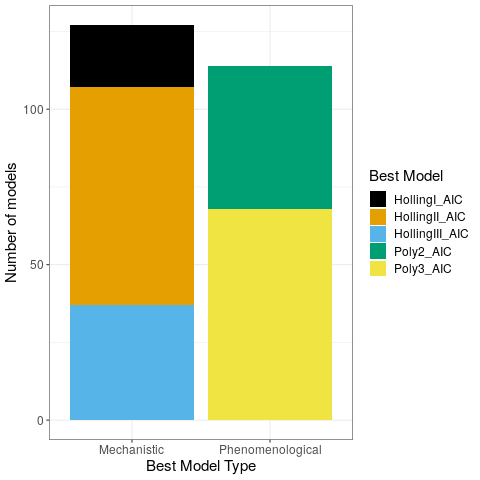
\includegraphics[width=5in]{../Results/Plots/modelbesttype}
    \caption{Number of models where the best type was phenomenological or mechanistic. Colour is the model. n=241}
    \label{fig:modelbesttype}
\end{figure}



The distribution of the best model was not best described by a uniform distribution but the distribution of the best model type was  (Table\ref{chitable}),
\input{../Results/Tables/output_chitable_latex}
%
%\subsection{Temperature and Best Model}
%The best model did not affect which model was the best.
\subsection{Temperature and Parameter Values}
The consumer temperatures are associated with the search rate and handling time (Figure \ref{fig:tempparam},Table \ref{Paramtemp}) % stats
\input{../Results/Tables/output_temp_con_latex}
The search rate is smaller and less varied at intermediate temperatures, however at very low and very high temperatures, the temperature is very varied and can be very high. There is a weak negative correlation. The handling time shows a weak positive correlation with consumer temperature.
%stats
\begin{figure}[ht]
\centering
\subfloat[Consumer temperature and log search rate for type I Holling model]{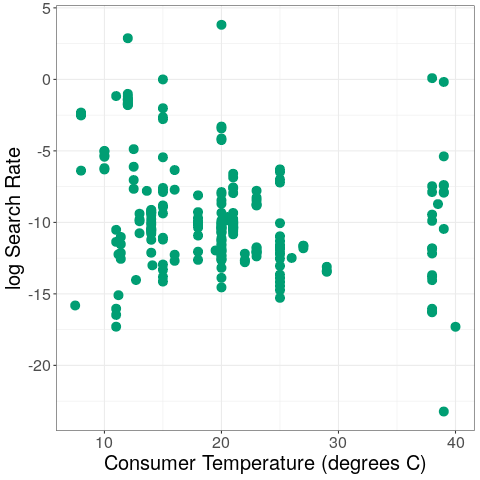
\includegraphics[width = 2.5in]{../Results/Plots/plot1conA}}\\
\subfloat[Consumer temperature with log search rate for type II Holling model]{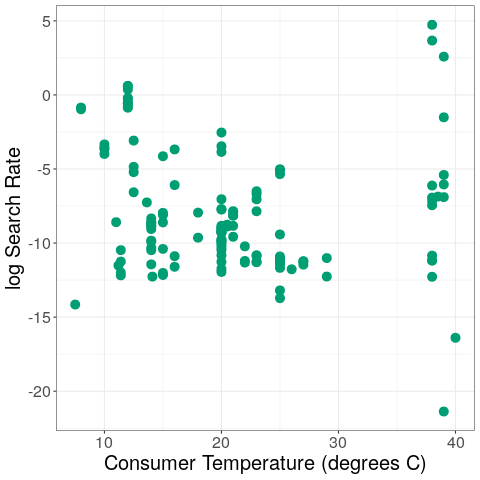
\includegraphics[width = 2.5in]{../Results/Plots/plot2conA}}
\subfloat[Consumer temperature with log handling time for type II Holling model]{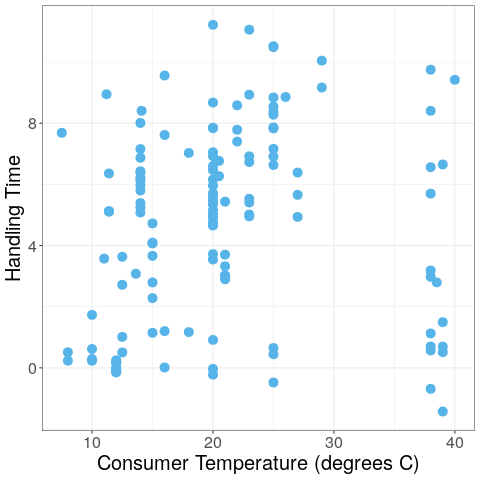
\includegraphics[width = 2.5in]{../Results/Plots/plot2conH}} \\
\subfloat[Resource temperature with log search rate for type III Holling model]{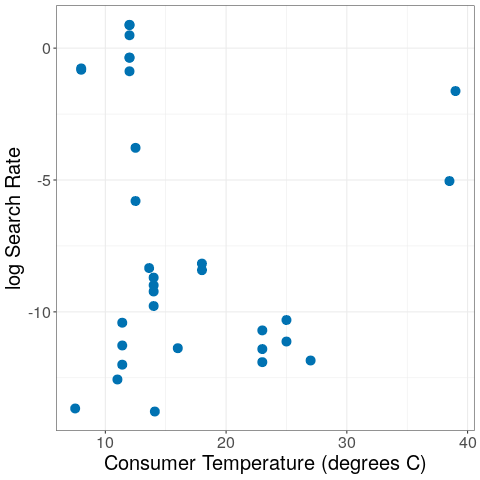
\includegraphics[width = 2.5in]{../Results/Plots/plot3conA}}
\subfloat[Consumer temperature with log handling time for type III Holling model]{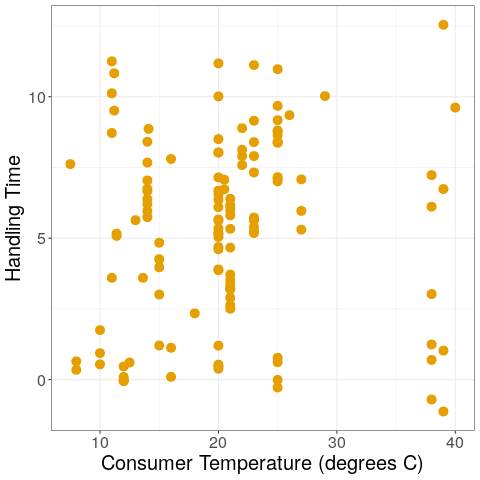
\includegraphics[width = 2.5in]{../Results/Plots/plot3conH}}
\caption{Logged parameter values and Consumer temperature for Type I, Type II and Type II Holling Models.}
\label{fig:tempparam}
\end{figure}

\section{Discussion}
%significance? 
\section{Conclusion}
%answer question

\clearpage{}


\begin{enumerate}
\item A citation command in parentheses: \parencite{hollingsawfly1959}.
\item A citation command for use in the flow of text: As \textcite{Holling1966} said \dots
\item A citation command which automatically switches style depending on location and the option setting in the package declaration (see line 12 in the LaTeX source code). In this case, it produces a citation in parentheses: \autocite{hollingsawfly1959}.
\end{enumerate}


\clearpage{}
%
% ---- Bibliography ----
%
% BibTeX users should specify bibliography style 'splncs04'.
% References will then be sorted and formatted in the correct style.
%

% Find from the left the folder bibliography/ and locate first.bib. you
% can generate your bibtex references using citethisforme and paste it inside the first.bib file
% to cite a bibliography, use \parencite{bisht_hinrichs_skrupsky_venkatakrishnan_2014} (example)
% those are citations embedded to texts
% please check out https://www.latex-tutorial.com/tutorials/bibtex/
\printbibliography
%\bibliography{references.bib}
%\bibliographystyle{plain}

\end{document}

